%%%%%%%%%%%%%%%%%%%%%%%%%%%%%%%%%%%%%%%%%%%%%%%%%%%%%%%%%%%%%%%%%%%%%%%%%%%%%%%%
%2345678901234567890123456789012345678901234567890123456789012345678901234567890
%        1         2         3         4         5         6         7         8

\documentclass[letterpaper, 10 pt, conference]{ieeeconf}  % Comment this line out
% if you need a4paper
%\documentclass[a4paper, 10pt, conference]{ieeeconf}      % Use this line for a4
% paper

\IEEEoverridecommandlockouts                              % This command is only
% needed if you want to
% use the \thanks command
\overrideIEEEmargins
% See the \addtolength command later in the file to balance the column lengths
% on the last page of the document

\usepackage[utf8]{inputenc}
\usepackage[T1]{fontenc}

% The following packages can be found on http:\\www.ctan.org
%\usepackage{graphics} % for pdf, bitmapped graphics files
%\usepackage{epsfig} % for postscript graphics files
%\usepackage{mathptmx} % assumes new font selection scheme installed
%\usepackage{mathptmx} % assumes new font selection scheme installed
\usepackage{amsmath}
%\usepackage{amssymb}  % assumes amsmath package installed
\usepackage{listings}
\usepackage{color}
\definecolor{dkgreen}{rgb}{0,0.6,0}
\definecolor{gray}{rgb}{0.5,0.5,0.5}
\definecolor{mauve}{rgb}{0.58,0,0.82}
\lstset{frame=tb,
    language=Python,
    aboveskip=3mm,
    belowskip=3mm,
    showstringspaces=false,
    columns=flexible,
    basicstyle={\small\ttfamily},
    numbers=none,
    numberstyle=\tiny\color{gray},
    keywordstyle=\color{blue},
    commentstyle=\color{dkgreen},
    stringstyle=\color{mauve},
    breaklines=true,
    breakatwhitespace=true,
    tabsize=3
}
\usepackage{graphicx}
\graphicspath{ {images} }

%%%%%%%%%%%%%%%%

\title{\LARGE \bf Lab 1 - Report}

\author{Shun Ueda}

\begin{document}
    \maketitle
    \thispagestyle{empty}
    \pagestyle{empty}


    \section{Excercise 1}
    For excerise 1 and 3, following functions are implemented.

    \begin{lstlisting}[label={lst:lstlisting}]
def sense(x):
    return x

def simulate(Δt, x, dx):
    x += Δt * dx
    return x
    \end{lstlisting}

    Control function is implemented as follows.

    \begin{lstlisting}[label={lst:lstlisting1}]
import numpy as np

def control(t, y):
    ux = -4 * sin(t)
    uy = 2 * cos(t)
    return np.array([ux, uy])
    \end{lstlisting}

    Since the major and minor axis are set to 4m and 2m respectively, we know that the functoin takes the form of $ux = 4 \sin(t)$ and $uy = 2 \cos(t)$.
    Moreover, since the path is counterclockwise, we adjust the function to $ux = -4 \sin(t)$ and $uy = 2 \cos(t)$.
    By observing figure $2.11$ we can see that the initial point is shifted right to 7, thus at $[7, 2]$.
    We can plot the path of the robot by using the following code.
    \begin{lstlisting}[label={lst:lstlisting2}]
from numpy import linspace, array, copy

tf = 2 * np.pi
Δt = 0.1
time = linspace(0., tf, int(tf / Δt) + 1)

# Initial conditions
x = array([7., 2.])
x_log = [copy(x)]

for t in time:
    y = sense(x)
    u = control(t, y)
    x = simulate(Δt, x, u)
    x_log.append(copy(x))
x_log = array(x_log)
    \end{lstlisting}
    \begin{lstlisting}[label={lst:lstlisting3}]
from matplotlib.pyplot import grid, plot, show

# Plotting
grid()
# Path of the robot
plot(x_log[:, 0], x_log[:, 1], 'r--')
show()
    \end{lstlisting}
    This will result in the following plot.
    \begin{center}
        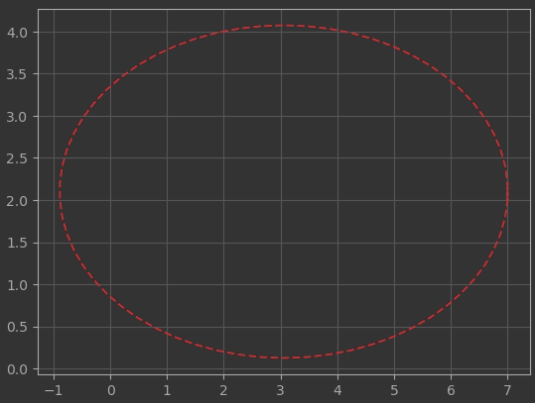
\includegraphics[scale=0.4]{exercise-1}
    \end{center}


    \section{Excercise 3}
    By using the formula $ux = \sin(t), uy = a\cos(bt)$, we obtain our control function as follows.
    \begin{lstlisting}[label={lst:lstlisting4}]
import numpy as np

def control(t, y):
    ux = sin(t)
    uy = 2 * cos(2 * t)
    return np.array([ux, uy])
    \end{lstlisting}
    The plotting is done in the same way as in exercise 1.
    Plot is shown below.
    \begin{center}
        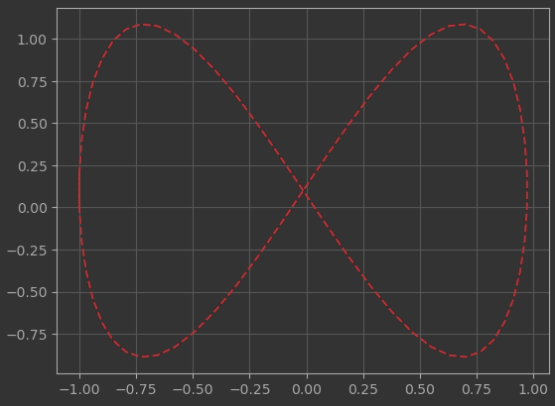
\includegraphics[scale=0.4]{exercise-2}
    \end{center}


    \section{Excercise 4}
    Control function is set to a regular cirtular path.
    \begin{lstlisting}[label={lst:lstlisting5}]
def control(t, y):
    ux = sin(t)
    uy = cos(t)
    return np.array([ux, uy])
    \end{lstlisting}

    \subsection{Constant Wind}
    We will modify the simulate function to include wind.
    \begin{lstlisting}[label={lst:lstlistin6}]
def simulate(Δt, x, dx, w):
    x += Δt * (dx + w)
    return x
    \end{lstlisting}

    \begin{lstlisting}[label={lst:lstlistin7}]
from numpy import linspace, array, copy

tf = 2 * np.pi
Δt = 0.1
time = linspace(0., tf, int(tf / Δt) + 1)
w = array([0.1, 0.1]) // contant wind

# Initial conditions
x = array([0., 0.])
x_log = [copy(x)]

for t in time:
    y = sense(x)
    u = control(t, y)
    x = simulate(Δt, x, u, w)
    x_log.append(copy(x))

x_log = array(x_log)
    \end{lstlisting}
    This will result in the following plot.
    \begin{center}
        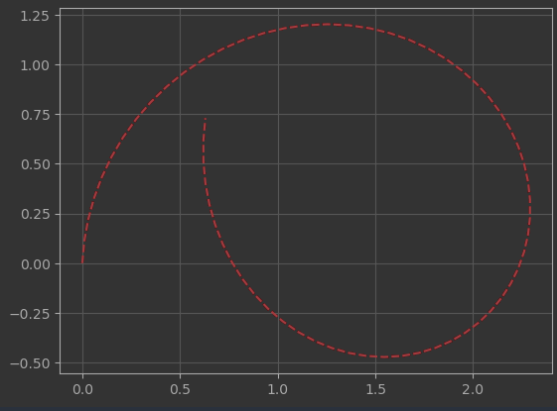
\includegraphics[scale=0.4]{exercise-4-1}
    \end{center}

    \subsection{Random Wind (\mu = 0, \sigma = 0.1)}
    We will modify the simulate function to include random wind.
    \begin{lstlisting}[label={lst:lstlistin8}]
def simulate(Δt, x, dx, mean_wind, std_dev):
    random_wind = np.random.normal(mean_wind, std_dev, 2)
    x += Δt * (dx + random_wind)
    return x
    \end{lstlisting}

    \begin{lstlisting}[label={lst:lstlistin9}]
from numpy import linspace, array, copy

tf = 2 * np.pi
Δt = 0.1
time = linspace(0., tf, int(tf / Δt) + 1)
mean_wind = 0.0
std_dev = 0.1

# Initial conditions
x = array([0., 0.])
x_log = [copy(x)]

for t in time:
    y = sense(x)
    u = control(t, y)
    x = simulate(Δt, x, u, mean_wind, std_dev)
    x_log.append(copy(x))

x_log = array(x_log)
    \end{lstlisting}
    This will result in the following plot.
    \begin{center}
        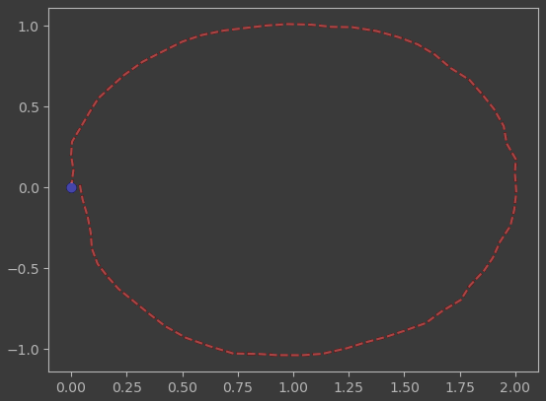
\includegraphics[scale=0.4]{exercise-4-2}
    \end{center}

%    \begin{lstlisting}[label={lst:}]
%from matplotlib.pyplot import grid, plot, show
%
%# Plotting
%grid()
%# Path of the robot
%plot(x_log[:, 0], x_log[:, 1], 'r--')
%show()
%    \end{lstlisting}
\end{document}
